%! Author = kyoto
%! Date = 08.03.2022


\section{Задание}
Реализовать консольное приложение, которое реализует управление коллекцией объектов в интерактивном режиме.
В коллекции необходимо хранить объекты класса Movie, описание которого приведено ниже.\\
Разработанная программа должна удовлетворять следующим требованиям:\\
\\
Класс, коллекцией экземпляров которого управляет программа, должен реализовывать сортировку по умолчанию.\\
Все требования к полям класса (указанные в виде комментариев) должны быть выполнены.\\
Для хранения необходимо использовать коллекцию типа java.util.PriorityQueue\\
При запуске приложения коллекция должна автоматически заполняться значениями из файла.\\
Имя файла должно передаваться программе с помощью: переменная окружения.\\
Данные должны храниться в файле в формате json\\
Чтение данных из файла необходимо реализовать с помощью класса java.util.Scanner\\
Запись данных в файл необходимо реализовать с помощью класса java.io.FileOutputStream\\
Все классы в программе должны быть задокументированы в формате javadoc.\\
Программа должна корректно работать с неправильными данными (ошибки пользовательского ввода, отсутсвие прав доступа к файлу и т.п.).\\
В интерактивном режиме программа должна поддерживать выполнение следующих команд:\\
\\
help : вывести справку по доступным командам\\
info : вывести в стандартный поток вывода информацию о коллекции (тип, дата инициализации, количество элементов и т.д.)\\
show : вывести в стандартный поток вывода все элементы коллекции в строковом представлении\\
add \{element\} : добавить новый элемент в коллекцию\\
update id \{element\} : обновить значение элемента коллекции, id которого равен заданному\\
remove\_by\_id id : удалить элемент из коллекции по его id\\
clear : очистить коллекцию\\
save : сохранить коллекцию в файл\\
execute\_script file\_name : считать и исполнить скрипт из указанного файла. В скрипте содержатся команды в таком же виде, в котором их вводит пользователь в интерактивном режиме.\\
exit : завершить программу (без сохранения в файл)\\
add\_if\_min \{element\} : добавить новый элемент в коллекцию, если его значение меньше, чем у наименьшего элемента этой коллекции\\
remove\_greater \{element\} : удалить из коллекции все элементы, превышающие заданный\\
remove\_lower \{element\} : удалить из коллекции все элементы, меньшие, чем заданный\\
remove\_all\_by\_oscars\_count oscarsCount : удалить из коллекции все элементы, значение поля oscarsCount которого эквивалентно заданному\\
remove\_any\_by\_director director : удалить из коллекции один элемент, значение поля director которого эквивалентно заданному\\
print\_field\_descending\_oscars\_count : вывести значения поля oscarsCount всех элементов в порядке убывания\\
Формат ввода команд:\\
Все аргументы команды, являющиеся стандартными типами данных (примитивные типы, классы-оболочки, String, классы для хранения дат), должны вводиться в той же строке, что и имя команды.\\
Все составные типы данных (объекты классов, хранящиеся в коллекции) должны вводиться по одному полю в строку.\\
При вводе составных типов данных пользователю должно показываться приглашение к вводу, содержащее имя поля (например, "Введите дату рождения:")\\
Если поле является enum'ом, то вводится имя одной из его констант (при этом список констант должен быть предварительно выведен).\\
При некорректном пользовательском вводе (введена строка, не являющаяся именем константы в enum'е; введена строка вместо числа; введённое число не входит в указанные границы и т.п.) должно быть показано сообщение об ошибке и предложено повторить ввод поля.\\
Для ввода значений null использовать пустую строку.\\
Поля с комментарием ``Значение этого поля должно генерироваться автоматически'' не должны вводиться пользователем вручную при добавлении.\\

\newpage

\section{Описание хранимых в коллекции классов}
\noindent\texttt{рublic class Movie \{ \\
    private long id; //Значение поля должно быть больше 0, Значение этого поля должно быть уникальным, Значение этого поля должно генерироваться автоматически\\
    private String name; //Поле не может быть null, Строка не может быть пустой\\
    private Coordinates coordinates; //Поле не может быть null\\
    private java.util.Date creationDate; //Поле не может быть null, Значение этого поля должно генерироваться автоматически\\
    private long oscarsCount; //Значение поля должно быть больше 0\\
    private MovieGenre genre; //Поле может быть null\\
    private MpaaRating mpaaRating; //Поле может быть null\\
    private Person director; //Поле может быть null\\
    \} \\
    \\
    public class Coordinates \{ \\
    private Double x; //Значение поля должно быть больше -312, Поле не может быть null\\
    private Integer y; //Значение поля должно быть больше -901, Поле не может быть null\\
    \} \\
    \\
    public class Person \{ \\
    private String name; //Поле не может быть null, Строка не может быть пустой\\
    private double height; //Значение поля должно быть больше 0\\
    private Color eyeColor; //Поле может быть null\\
    private Color hairColor; //Поле не может быть null\\
    private Country nationality; //Поле не может быть null\\
    private Location location; //Поле может быть null\\
    \} \\
    \\
    public class Location \{ \\
    private Double x; //Поле не может быть null\\
    private double y;\\
    private Double z; //Поле не может быть null\\
    private String name; //Длина строки не должна быть больше 233, Поле может быть null\\
    \} \\
    \\
    public enum MovieGenre \{ \\
    ACTION,\\
    DRAMA,\\
    ADVENTURE;\\
    \} \\
    \\
    public enum MpaaRating \{ \\
    PG,\\
    PG\_13,\\
    R,\\
    NC\_17;\\
    \} \\
    \\
    public enum Color \{ \\
    BLUE,\\
    ORANGE,\\
    WHITE,\\
    BROWN;\\
    \} \\
    \\
    public enum Color \{ \\
    GREEN,\\
    BLACK,\\
    YELLOW;\\
    \} \\
    \\
    public enum Country \{ \\
    GERMANY,\\
    NORTH\_KOREA,\\
    JAPAN;\\
    \} \\
}
\newpage


\section{Диаграмма классов}

\begin{figure}[H]
    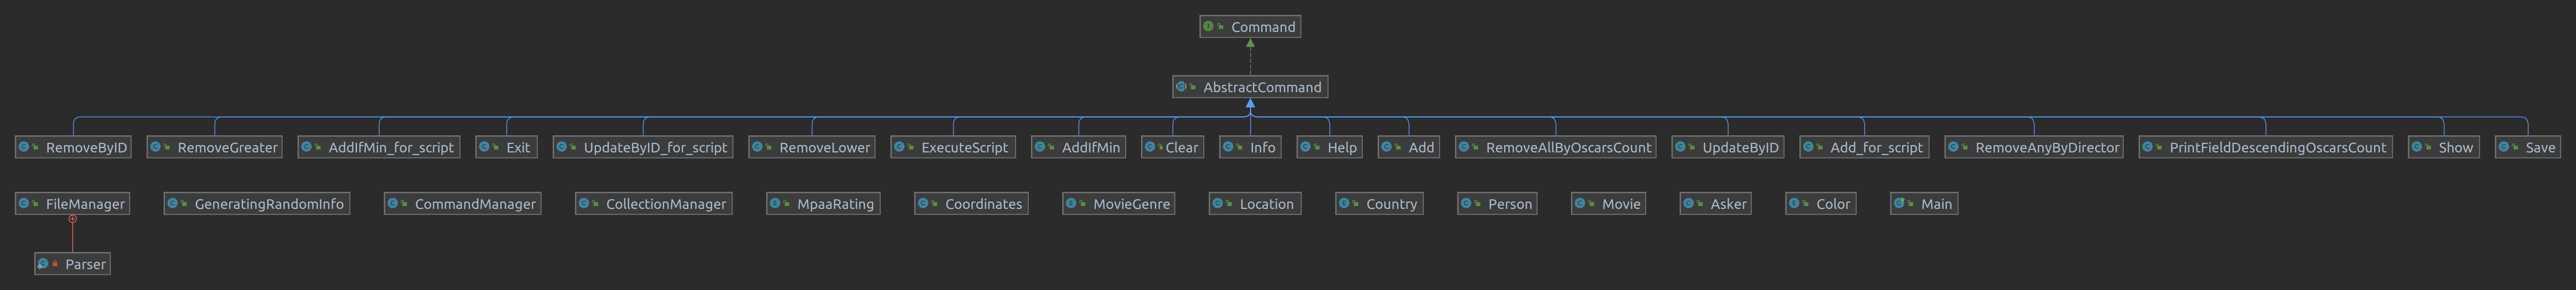
\includegraphics[scale=0.07]{img/diagram}
\end{figure}

\section{Исходный код}
\url{https://github.com/Kyoto67/VT_labs_1/tree/Programming_lab5}